%%%%%%%%%%%%%%%%%%%%%%%%%%%%%%%%%%%%%%%%%%%%%%%%%%%%%%%
%                   File: OSAmeetings.tex             %
%                  Date: March 21, 2007  MSD          %
%                                                     %
%     For preparing LaTeX manuscripts for submission  %
%       submission to OSA meetings and conferences    %
%                                                     %
%       (c) 2007 Optical Society of America           %
%%%%%%%%%%%%%%%%%%%%%%%%%%%%%%%%%%%%%%%%%%%%%%%%%%%%%%%

\documentclass[letterpaper,10pt]{article}
\usepackage{osameet2}

%% standard packages and arguments should be modified as needed

\usepackage{amsmath,amssymb}

% \bibliography{paper}
% \bibliographystyle{osajnl}


%\usepackage[pdftex,colorlinks=true,bookmarks=false,citecolor=blue,urlcolor=blue]{hyperref} %pdflatex
\usepackage[colorlinks=true,bookmarks=false,citecolor=blue,urlcolor=blue]{hyperref} %latex w/dvips


\begin{document}

\title{Three-dimensional fluorophore orientation imaging with polarized multiview microscopy}

\author{Talon Chandler,${}^{1,*}$ Min Guo,${}^2$ Shalin Mehta,${}^{1,3,4}$ Abhishek Kumar,${}^2$\\ Hari Shroff,${}^{2,5}$ Rudolf Oldenbourg,${}^{3,6}$ Patrick J. La Rivi\`ere${}^{1,5}$}

\address{${}^1$Department of Radiology, University of Chicago, Chicago, Illinois 60637, USA.\\ ${}^2$Section on High Resolution Optical Imaging, National Institute of Biomedical Imaging\\ and Bioengineering, National Institutes of Health, Bethesda, Maryland 20892, USA.\\ ${}^3$Bell Center, Marine Biological Laboratory, Woods Hole, Massachusetts 02543, USA.\\ ${}^4$(present address) Chan Zuckerberg Biohub, San Francisco, California 94158, USA.\\ ${}^5$Whitman Center, Marine Biological Laboratory, Woods Hole, Massachusetts 02543, USA.\\ ${}^6$Department of Physics, Brown University, Providence, Rhode Island 02912, USA.}
\email{${}^*$talonchandler@talonchandler.com} %% email address is required

\begin{abstract}
  We show that polarized fluorescence microscopes make band-limited measurements
  in the angular frequency domain. We use this result to propose and demonstrate
  efficient algorithms for reconstructing three-dimensional fluorophore
  orientations from polarized multiview microscope data.
\end{abstract}

\ocis{180.2520 Fluorescence microscopy, 260.5430 Polarization}

\section{Introduction}


\section{Theory}
\cite{chandler}
\cite{barrett} 
\section{Results}

\begin{figure}[htbp]
  \centering
  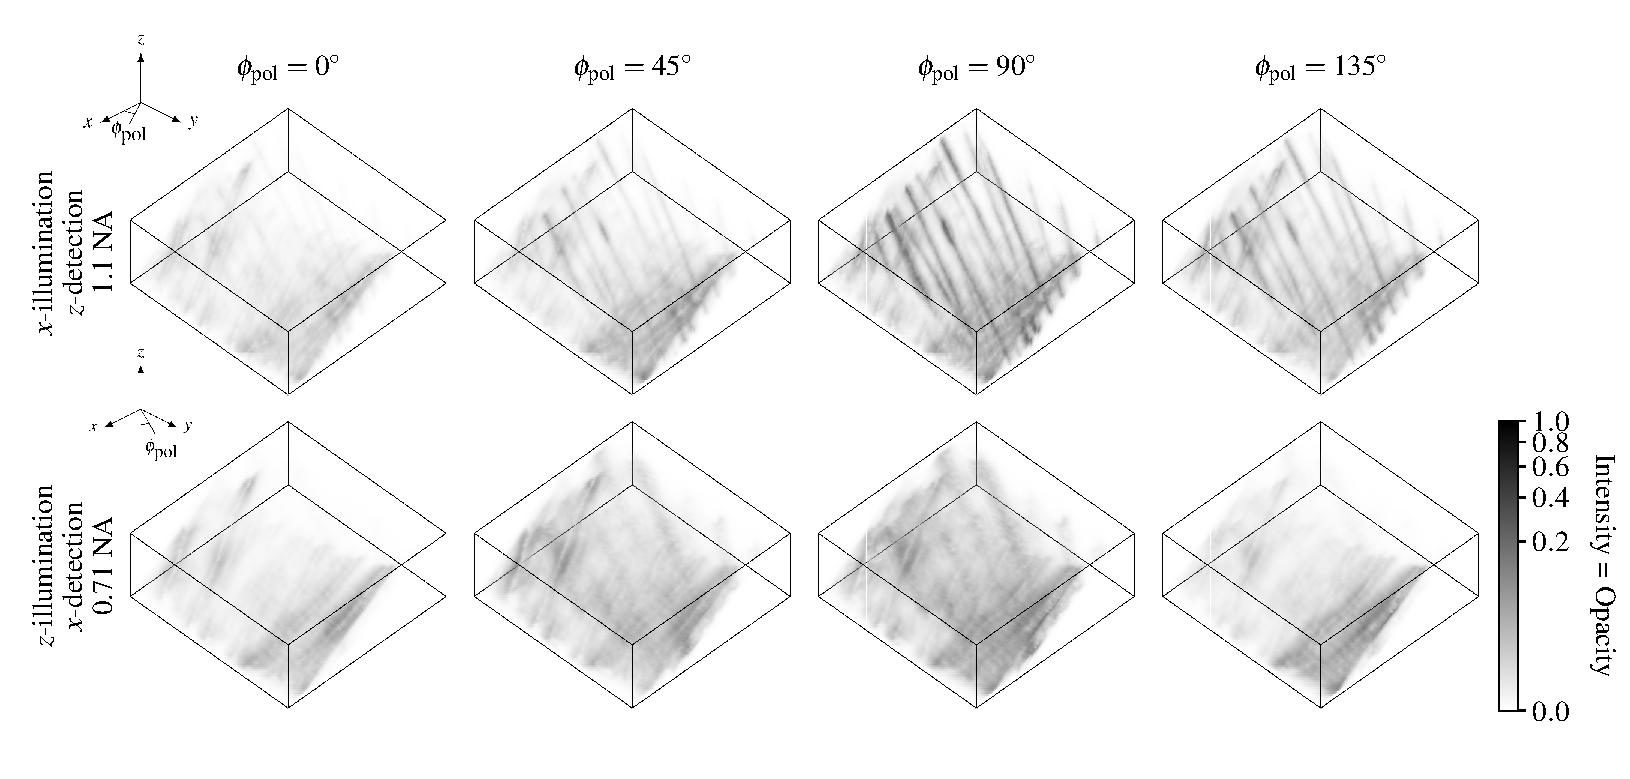
\includegraphics[width=17cm]{figs/roi2/data.pdf}
\caption{Data.}
\end{figure}

\begin{figure}[htbp]
  \centering
  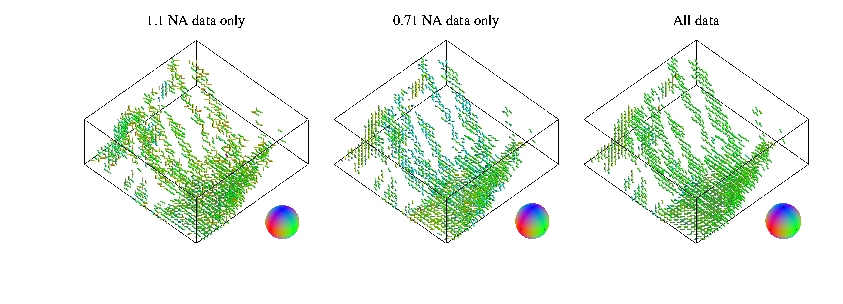
\includegraphics[width=17cm]{figs/roi2/recon.pdf}
\caption{Reconstruction.}
\end{figure}



\bibliography{abstract}{}
\bibliographystyle{osajnl}

\end{document}
